\documentclass{article}[12pt]

\usepackage[utf8]{inputenc}
\usepackage{amsfonts,amssymb,amsmath,subfigure}
\usepackage[pdftex]{graphicx}
\usepackage{epstopdf}
\usepackage{vmargin}
\usepackage{comment}
\usepackage{tikz,multicol}

\usepackage{algorithm}
\usepackage[noend]{algpseudocode}
\usepackage{tcolorbox}

\newtcolorbox{mybox}[3][]
{
  colframe = #2!25,
  colback  = #2!10,
  coltitle = #2!20!black,  
  title    = {#3},
  #1,
}


\newcommand*\Let[2]{\State #1 $\gets$ #2}
\algrenewcommand\algorithmicrequire{\textbf{Precondition:}}
\algrenewcommand\algorithmicensure{\textbf{Postcondition:}}




\excludecomment{solution}
%\includecomment{solution}

\title{IF111 - Algorithmes et structures de données\\EI3 - Structures de données et arbres de recherche}
\date{\texttt{rfosse@labri.fr}}
\author{Rohan Fossé}
\begin{document}



\maketitle{}

\section*{Insertion dans les ABR, Tas min et AVL}
    Soit la liste de clés L = (6, 11, 26, 28, 2, 3). Pour chacune des structures, en partant d’un arbre binaire vide, vous devez dessiner l’arbre après chacune des insertions des éléments de la liste L.
    \begin{enumerate}
        \item Arbre binaire de recherche (ABR)
        \item Tas min
        \item AVL
    \end{enumerate}

    
    
    
\section*{Tas binaire}
\begin{enumerate}
\item Dessiner un tas binaire max pour l'ensemble de clés $\{1,4,5,16,17,21\}$. Pour le même ensemble dessiner un tas binaire min.
\item Quels sont les nombres minimum et maximum d'éléments dans un tas de hauteur h?

\item Démontrer que un tas avec $n$ sommets a hauteur $\lfloor$log(n)$\rfloor$.
\end{enumerate}
\section*{Arbres binaires de recherche}
\begin{enumerate}
\item Dessiner des arbres binaires de recherche de hauteur respectivement 2, 3 et 6 pour le même ensemble de clés $\{1,4,5,10,16,17,21\}$.
\item Dessiner tous les arbres binaires de recherche valués sur $V = \{10, 20, 30, 40\}$ ayant 20 comme valeur à la racine.
\item Quel parcours de l'arbre binaire de recherche permet d'afficher toutes les clés de l'arbre triées?
\item On suppose que des entiers compris entre 1 et 1000 sont disposés dans un arbre binaire de recherche et que l'on souhaite trouver le nombre 363. Parmi les séquences suivantes, lesquelles ne pourraient pas être la suite de sommets parcourus?
\begin{enumerate}
\item 2, 252, 401, 398, 330, 344, 397, 363
\item 924, 220, 911, 244, 898, 258, 362, 363
\item 925, 202, 911, 240, 912, 245, 363
\end{enumerate}

\item Ajouter successivement à l’arbre binaire dessiné sur la Fig. 1 les valeurs : 9, 14, 16, 6, 23, 5.
\begin{figure}[hbtp] 
  \centering
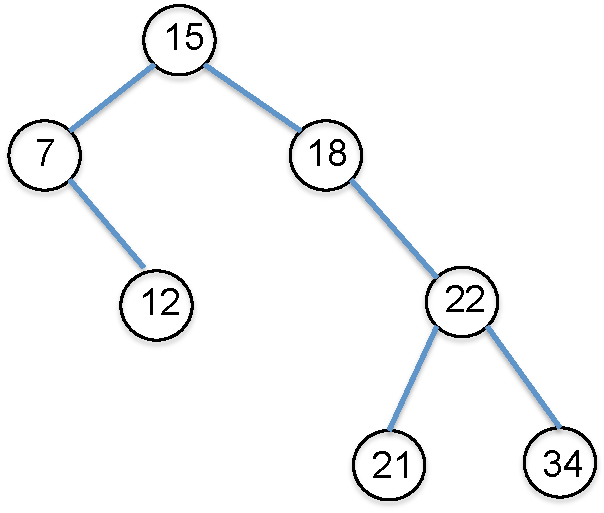
\includegraphics[scale =0.5] {ABR.pdf}\label{fig:abr} \caption{Arbre binaire de recherche}
\end{figure}
\item Soit un arbre binaire de recherche T dont les clés sont distinctes. Montrer que si le sous-arbre droit d'un noeud $x$ dans $T$ est vide et que $x$ a un successeur $y$, alors $y$ est l'ancêtre le plus bas de $x$ dont le fils gauche est aussi un ancêtre de $x$ (Ne pas oublier que chaque noeud est son propre ancêtre).
\item Montrer que, si un noeud d'un arbre binaire de recherche a deux fils, alors son successeur n'a pas de fils gauche.
\end{enumerate}


\section*{Recherche dans un ABR}
\begin{enumerate}
    \item Écrire une fonction qui retourne true si l’ABR qui lui est passé en paramètre
est une feuille.
    \item  Écrire une fonction récursive qui affiche l’ABR qui lui est passé en para-
mètre, par ordre croissant des valeurs.
    \item Écrire une fonction récursive qui affiche l’ABR qui lui est passé en para-
mètre, par ordre décroissant des valeurs.
    \item Écrire une fonction qui retourne la hauteur de l’ABR qui lui est passé en
paramètre.
\item Écrire une fonction qui retourne le nombre de nœuds de l’ABR qui lui est
passé en paramètre.
\end{enumerate}

\section*{Suppression dans un arbre binaire de recherche}
Soit l’arbre binaire de recherche donné dans la figure 1
\begin{enumerate}
    \item Dessiner l’arbre après la suppression du noeud 18.
    \item  L’opération suppression est-elle ”commutative” au sens où la suppression de x puis de y dans un arbre binaire de recherche produit le même arbre que la suppression de y puis
de x.\\
Si oui dire pourquoi, sinon donner un contre exemple.
\end{enumerate}


\section*{Récursivité sur les arbres binaires de recherche}
On veut concevoir des algorithmes récursifs pour calculer des propriétés d'un arbre binaire donné en entrée. 
Les algorithmes peuvent utiliser les fonctions $estVide(T)$ qui retourne vrai si l'arborescence $T$ est vide,  $filsgauche(T)$ et $filsdroit(T)$ qui retournent respectivement le sous-arbre gauche et le sous-arbre droit de l'arbre $T$. Décrire l'idée des algorithmes et en écrire le pseudo-code.
\begin{enumerate}			
\item Concevoir un algorithme récursif, nommé $Hauteur(T)$, qui calcule la hauteur d'une arborescence binaire $T$ donnée en entrée. Si l'arborescence est vide l'algorithme retournera $-1$. L'algorithme s'appuie sur la technique diviser pour régner. 


			
	%\item Calculer la récurrence correspondante aux additions exécutées par l'algorithme $Hauteur(T)$ en considérant comme taille de %l'entrée le nombre de noeuds qui constituent l'arborescence binaire en entrée en considerant des arbres binaires complètes. Résoudre la récurrence \\
%			\begin{solution}  La récurrence est la suivante : \[A(n_T)=A(n_{filsgauche(T)})+A(n_{filsdroit(T)})+1 \  pour \  n_T>0 \  et \  A(0)=0.\]
%			\end{solution}
\item Concevoir un algorithme récursif qui calcule le nombre de feuilles d'une arborescence binaire donnée en entrée. 
	


\end{enumerate}

\section*{Parcours en largeur}
\begin{figure}[hbtp] 
  \centering
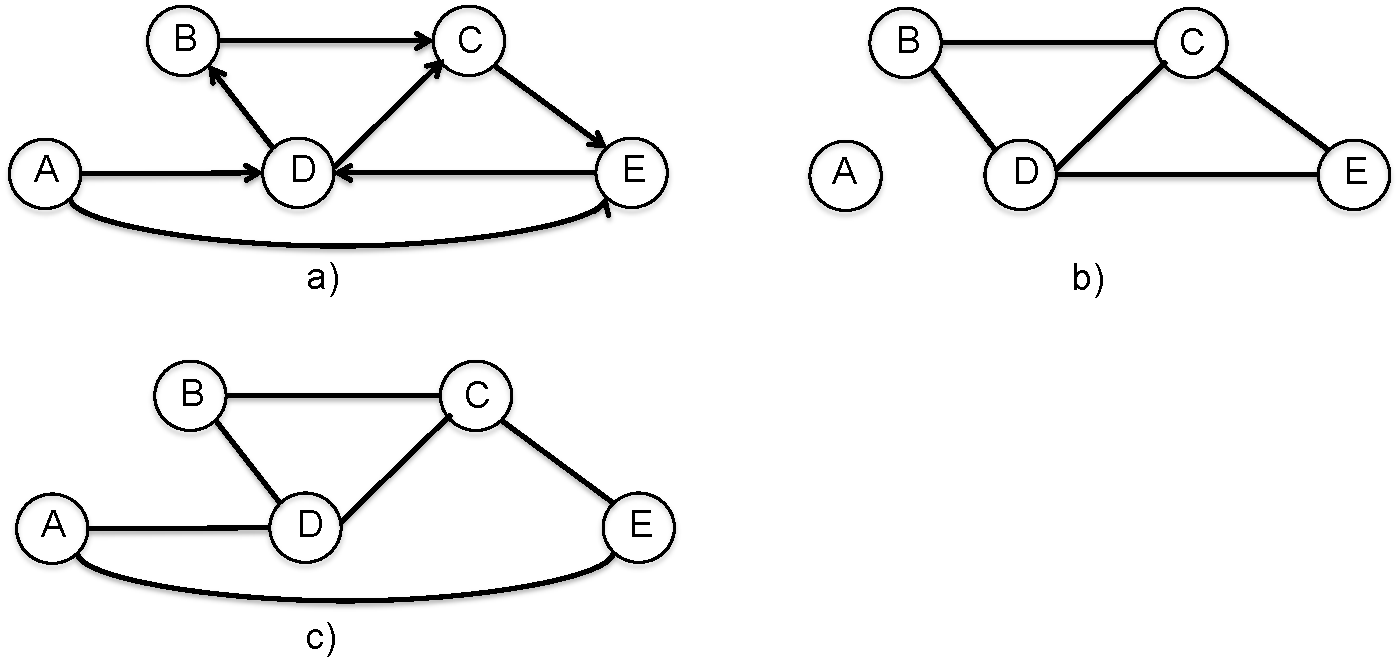
\includegraphics[scale =0.5] {graphes.pdf} \caption{Graphes.} \label{fig:graphes}
\end{figure}

\begin{enumerate}
\item Appliquer l’algorithme de parcours en largeur au graphe non orienté dans la Figure \ref{fig:graphes} (c) le sommet origine étant $A$.
\item Un graphe non orienté $G=(V,E)$ est dit \emph{connexe} si quels que soient les sommets $u$ et $v$ de $V$, il existe une chaîne reliant $u$ à $v$. Donner un exemple d'un graphe qui n'est pas connexe. Comment utiliser l’algorithme de parcours en largeur pour tester si un graphe non orienté est \emph{connexe}?
\end{enumerate}


\section*{Algorithme de Dijkstra}
On considère maintenant des graphes pondérés. Appliquer l'algorithme de Dijkstra au graphe dans la Figure \ref{fig:grapheDijkstra} pour calculer la plus courte distance de $A$ à $E$.

\begin{figure}[hbtp] 
  \centering
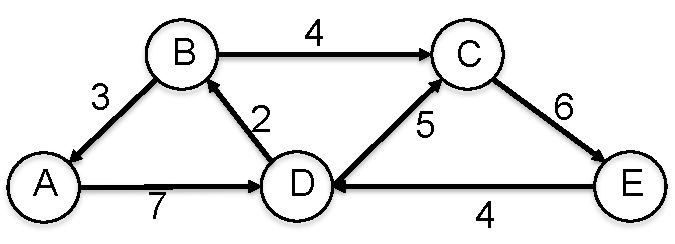
\includegraphics[scale =0.5] {graphe.pdf} \caption{Graphe pour Dijkstra.} \label{fig:grapheDijkstra}
\end{figure}

\section*{Algorithme de Connexité}
\begin{figure}[hbtp] 
  \centering
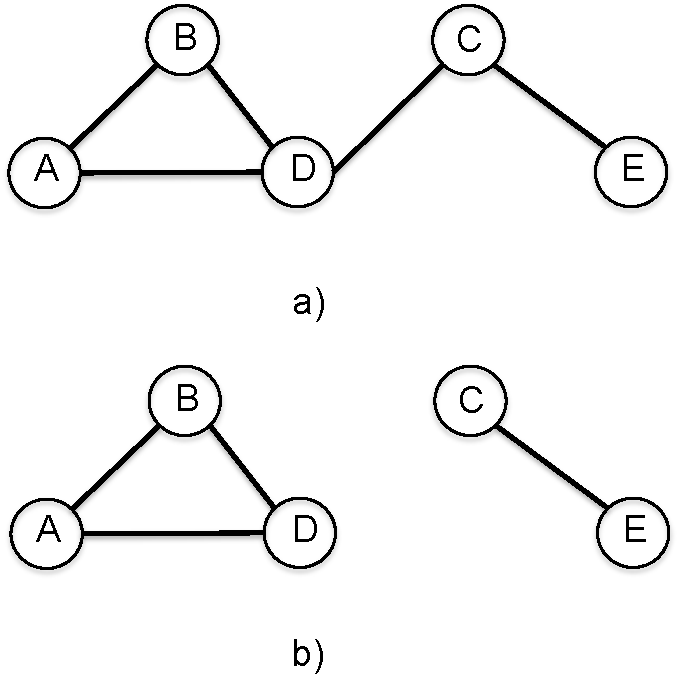
\includegraphics[scale =0.5] {grapheConnexe.pdf} \caption{Graphes} \label{fig:grapheConnexe}
\end{figure}

Un graphe est dit \emph{connexe} si pour toute paire de sommets s, t, il existe un chemin allant de s à t. Pour chaque graphe en Figure \ref{fig:grapheConnexe} dire s'il est connexe ou pas. Écrivez un algorithme qui teste si un graphe non orienté $G(V,E)$ est connexe ou non. \\ Donner la matrice d'adjacence et la liste d'adjacence des graphes en Figure \ref{fig:grapheConnexe}.

\section*{Composantes connexes}
Une composante connexe d’un graphe est un sous-graphe connexe tel que chaque sommet de la composante connexe n’est relié à aucun sommet n’appartenant pas à cette composante connexe. 
\begin{enumerate} 
\item Donnez la liste des composantes connexes pour chaque graphe G en Figure \ref{fig:grapheConnexe} .
\item Écrire un algorithme qui calcule la liste des composantes connexes d’un graphe non orienté. On pourra coder cette information en indiquant pour chaque sommet du graphe le numéro de la composante connexe à laquelle il appartient. On peut supposer que les sommets sont numérotés de $1$ à $n$. L'algorithme retournera un tableau où l'indice $i$ pour de $1$ à $n$ contiendra le numéro de la composante connexe à laquelle appartient le sommet $i$.


\item On considère le graphe G défini par la matrice d’adjacence suivante :
\[
\begin{pmatrix}
0 &0 &0 &0 &1& 0 & 0 & 0 \\
0 &0 &0 &0 &0& 0 & 1 & 1 \\
0 &0 &0 &0 &1& 1 & 0 & 0  \\
0 &0 &0 &0 &0& 0 & 0 & 0  \\
1 &0 &1 &0 &0& 1 & 0 & 0  \\
0 &0 &1 &0 &1& 0 & 0 & 0  \\
0 &1 &0 &0 &0& 0 & 0 & 1 \\
0 &1 &0 &0 &0& 0 & 1 & 0  \\
\end{pmatrix}
\]
Dessinez ce graphe et dire si c'est connexe.
\end{enumerate}
\section*{Récursivité sur les arbres}
\begin{enumerate}
\item Dessiner l'arborescence binaire ayant 10 noeuds \{0, 1, 2, ..., 9\}, telle que le parcours infixe et le parcours postfixe de cette arborescence produisent respectivement les suites suivantes : 9, 3, 1, 0, 4, 2, 6, 7, 8, 5 (infixe) et 9, 1, 4, 0, 3, 6, 7, 5, 8, 2 (postfixe). Dire quel est le raisonnement utilisé pour arriver à la solution.\\ Dire quelle est la hauteur du noeud 1 et 2 dans l'arborescence dessinée et quelle est la hauteur de l'arborescence elle même. \\

\item Ecrire la suite d'entiers obtenue par le parcours préfixe de l'arborescence obtenue dans la question precedente. Ecrire un algorithme recursif qui prend en entrée une arborescence et affiche les valeurs des n{\oe}uds dans l'ordre du parcours préfixe de l'arborescence. L' algorithme utilisera les fonctions $estVide(T)$ qui retourne vrai si l'arborescence $T$ est vide, $val(T$) qui retourne l'étiquette de la racine
d’un arbre non vide et $filsgauche(T)$ et $filsdroite(T)$ qui retournent respectivement la sous-arbre gauche et le sous-arbre droit de l'arborescence $T$.\\

\end{enumerate}



\end{document}